% Created 2024-08-23 Fri 13:57
% Intended LaTeX compiler: pdflatex
\documentclass[aspectratio=169,xcolor={dvipsnames,svgnames}]{beamer}
\usepackage[utf8x]{inputenc}
\usepackage[T1]{fontenc}
\usepackage{graphicx}
\usepackage{longtable}
\usepackage{wrapfig}
\usepackage{rotating}
\usepackage[normalem]{ulem}
\usepackage{amsmath}
\usepackage{amssymb}
\usepackage{capt-of}
\usepackage{hyperref}
\usepackage{minted}
\usepackage{libertine}
\usepackage[normalem]{ulem}
\usepackage{varwidth}
\usepackage[Export]{adjustbox}
%\usepackage{enumitem}
\graphicspath{ {./careful-Isaac-Images/} {./org-download-images/} }
\usepackage[date=year,%
backend=biber,%
style=alphabetic,%
maxnames=5,%
minnames=3,%
maxalphanames=4,%
minalphanames=3,%
backref=true,%
doi=false,%
isbn=false,%
url=false,%
eprint=false]{biblatex}
\DefineBibliographyStrings{english}{%
backrefpage  = {\lowercase{s}ee p.}, % for single page number
backrefpages = {\lowercase{s}ee pp.} % for multiple page numbers
}
\addbibresource{/home/bvraghav/bibliography.bib}
%% Math typesetting
%% --------------------------------
\usepackage{amsmath}
\usepackage{amssymb}
\usepackage{amsfonts}
\usepackage{bbold}
% Operators with limit-style sub and superscript
\DeclareMathOperator*{\E}{\mathbb{E}}
\hypersetup{%
colorlinks=true,%
allcolors=magenta,%
%linkbordercolor = {white},%
%<your other options...>,
}
\usetheme{boxes}
\usecolortheme{crane}
\usefonttheme{serif}
\useinnertheme{rectangles}
\useoutertheme{}
\date{}
\title{mca101 : computer graphics}
\subtitle{2d geometry representation}
\author{%
%\noindent{} \\[2em]
\normalsize Raghav B. Venkataramaiyer
}
\institute{%
CSED TIET Patiala India.
}
\date{\scriptsize \today}
\setbeamercolor{alerted text}{fg=red!80!black}
%% Setup outline at begin section
%% -------------------------------------------------------
\AtBeginSection[]               % Section
{
\begin{frame}{outline}
\tableofcontents[currentsection,hideallsubsections]
\end{frame}
}
\AtBeginSubsection[]            % SubSection
{
\begin{frame}{outline}
\tableofcontents[currentsection,currentsubsection,subsectionstyle=show/shaded/hide]
\end{frame}
}
\setbeamerfont{structure}{shape=\scshape,family=\sffamily}
\setbeamertemplate{section page}
{
\begin{centering}
\begin{beamercolorbox}[sep=12pt,center]{part title}
\usebeamerfont{section title}\insertsection\par
\end{beamercolorbox}
\end{centering}
}

\setbeamercovered{transparent}
\hypersetup{
 pdfauthor={B.V. Raghav},
 pdftitle={mca101 : computer graphics},
 pdfkeywords={},
 pdfsubject={},
 pdfcreator={Emacs 29.4 (Org mode 9.6.24)}, 
 pdflang={English}}
\begin{document}

\maketitle

\section{2d geometry --- introduction}
\label{sec:org5b8f4cc}

\subsection{Straight Lines}
\label{sec:org76c1fad}

\begin{frame}[label={sec:orgee07fde}]{\(y = mx + c\)}
\begin{align}
  \notag
  y = f(x) &= mx + c
\end{align}

\begin{center}
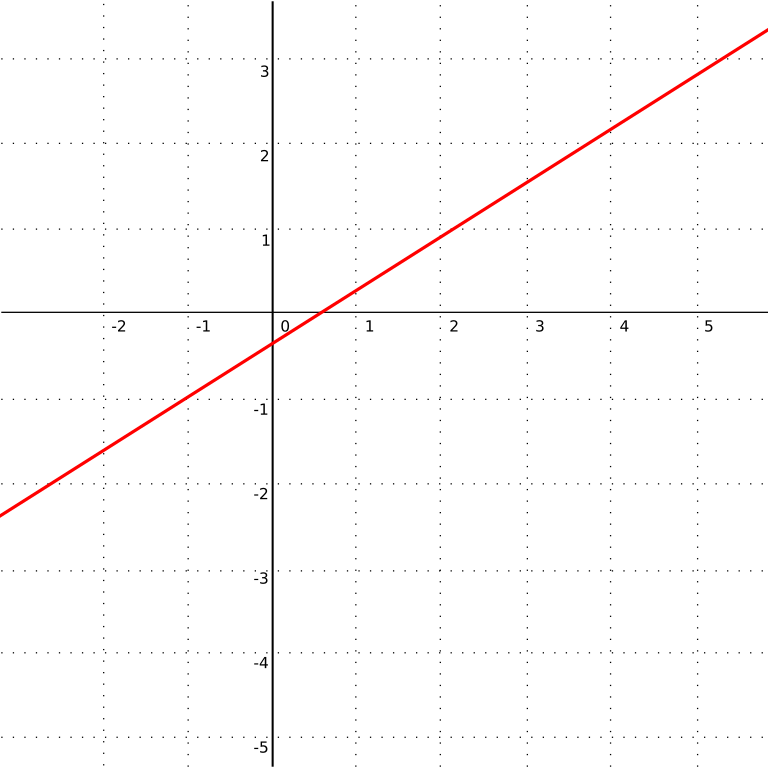
\includegraphics[width=0.3\linewidth]{images/st-line.png}
\end{center}
\end{frame}

\begin{frame}[label={sec:org7f9b56d}]{parametric form}
\begin{columns}
\begin{column}{.5\columnwidth}
For any two vectors \(\mathbf{u},\mathbf{v}\in V\), a
point on the line segment joining them is given
parameterised by \(t\in[0,1]\), as

\begin{align}
  \notag
  \mathbf{p} = f(t) &= (1-t)\mathbf{u} + t\mathbf{v}
\end{align}
\end{column}
\end{columns}
\end{frame}

\begin{frame}[label={sec:org112e5a4}]{parametric form}
\begin{columns}
\begin{column}{.5\columnwidth}
Any point on a line in the direction of unit vector
\(\mathbf{u}:\|\mathbf{u}\|_2^2=1\), and an incident
point \(\mathbf{p}_0\) may be given parameterised by
\(t\in\mathbb{R}\) as,

\begin{align}
  \notag
  \mathbf{p} = f(t) &= \mathbf{p}_0 + t\mathbf{u}
\end{align}
\end{column}
\end{columns}
\end{frame}

\begin{frame}[label={sec:org182415f}]{hesse normal form}
\begin{columns}
\begin{column}{.5\columnwidth}
\begin{center}
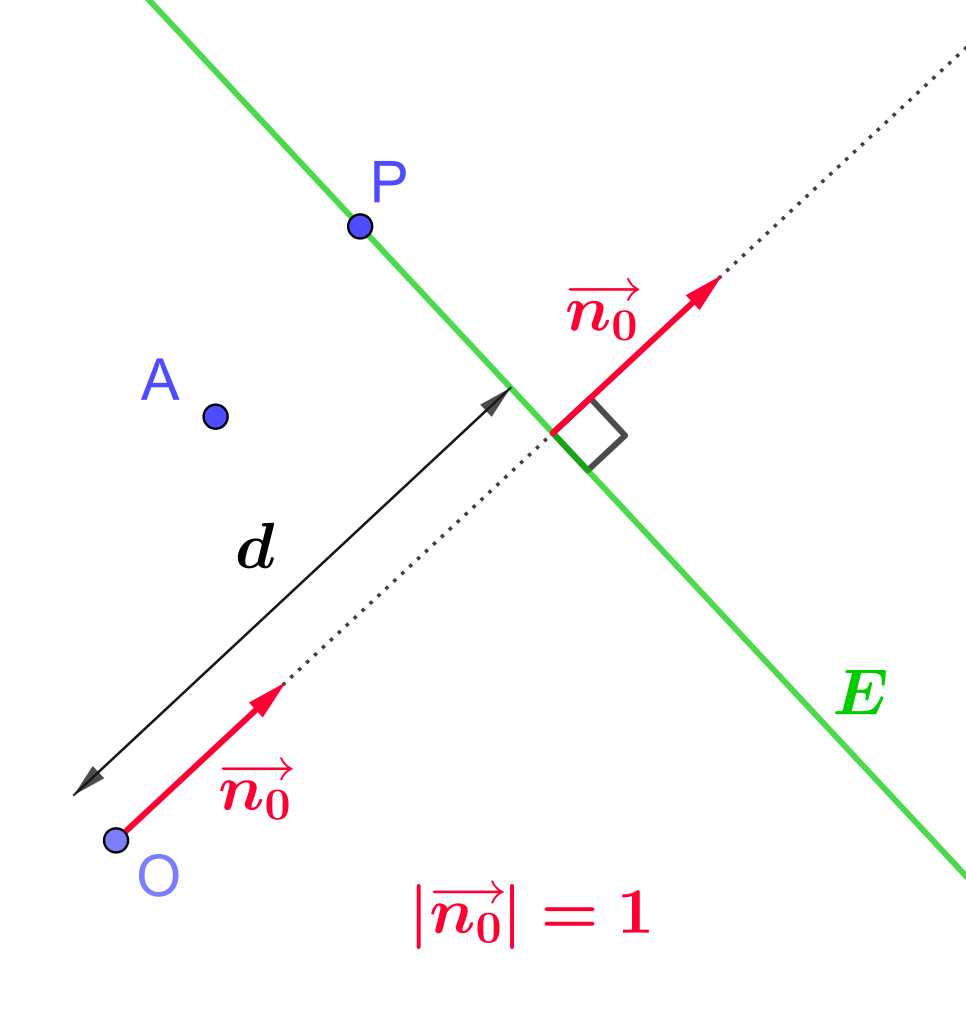
\includegraphics[width=0.7\linewidth]{images/Hesse_normalenform.svg.png}
\end{center}

Distance from the origin \(O\) to the line \(E\) calculated
with the Hesse normal form. Normal vector in red, line
in green, point O shown in blue.
\end{column}

\begin{column}{.6\columnwidth}
Given, \\[0pt]
Normal to the line
\(\mathbf{n}_0:\|\mathbf{n}_0\|_2^2=1\), and \\[0pt]
its distance from origin, \(d\);

\vspace{\baselineskip}
The point on the line is given implicitly as the locus
of all points \(\mathbf{p}\) that satisfy,

\begin{align}
  \notag
  \mathbf{n}_0 \cdot \mathbf{p} - d &= 0
\end{align}
\end{column}
\end{columns}
\end{frame}

\subsection{Conics}
\label{sec:org458f0d5}


\begin{frame}[label={sec:org3aea93e}]{circle}
\begin{columns}
\begin{column}{.4\columnwidth}
\begin{figure}[htbp]
\centering
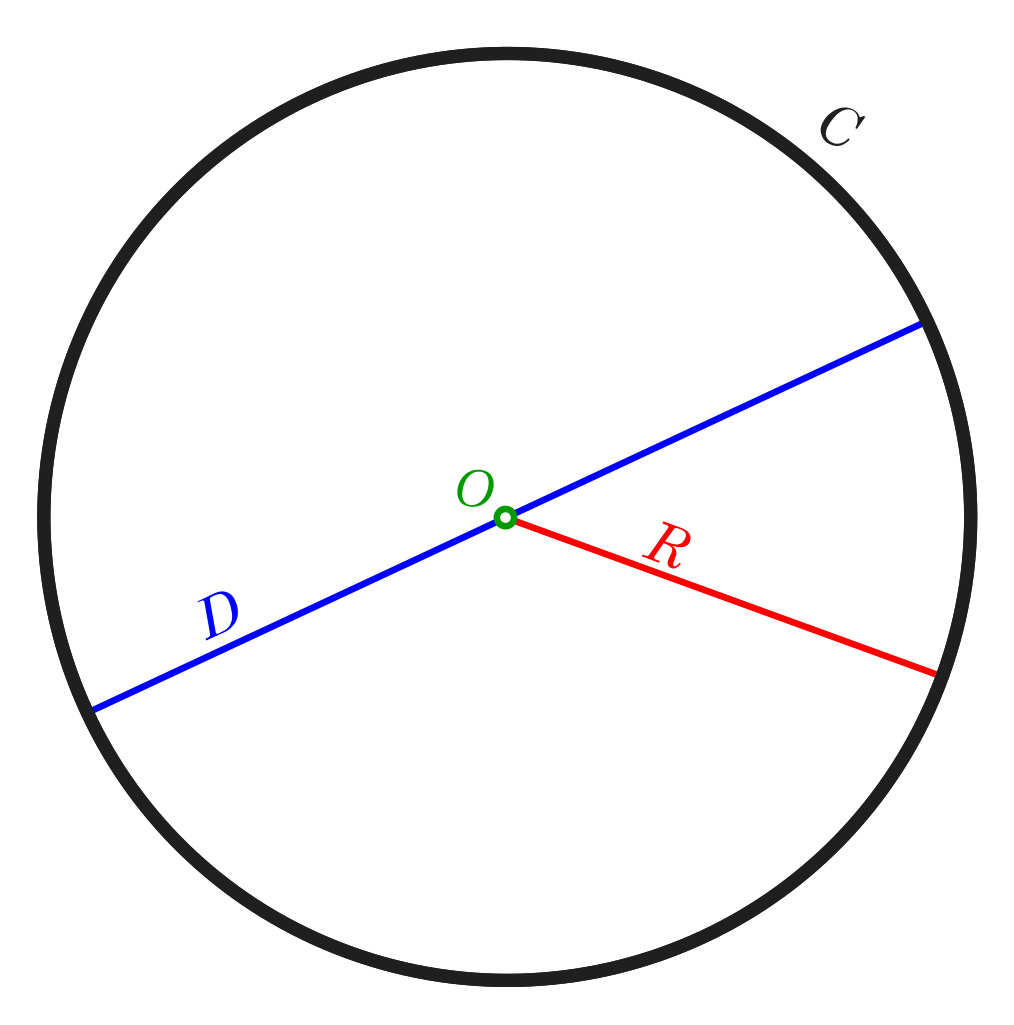
\includegraphics[width=.9\linewidth]{images/Circle-withsegments.svg.png}
\caption{Image Courtesy: \href{https://en.wikipedia.org/wiki/File:Circle-withsegments.svg}{Wikipedia}}
\end{figure}
\end{column}

\begin{column}{.6\columnwidth}
Implicit Form:
\begin{align}
  \notag
  f\left(\begin{matrix}x\\y\end{matrix}\right)
  &= x^2 + y^2 - r^2 = 0
\end{align}

Parametric Form:
\begin{align}
  \notag
  f(r,t)
  &= \begin{bmatrix}r\cos t\\r\sin t\end{bmatrix}
\end{align}
\end{column}
\end{columns}
\end{frame}
\begin{frame}[label={sec:org3fd2af4}]{ellipse}
\begin{columns}
\begin{column}{.4\columnwidth}
\begin{figure}[htbp]
\centering
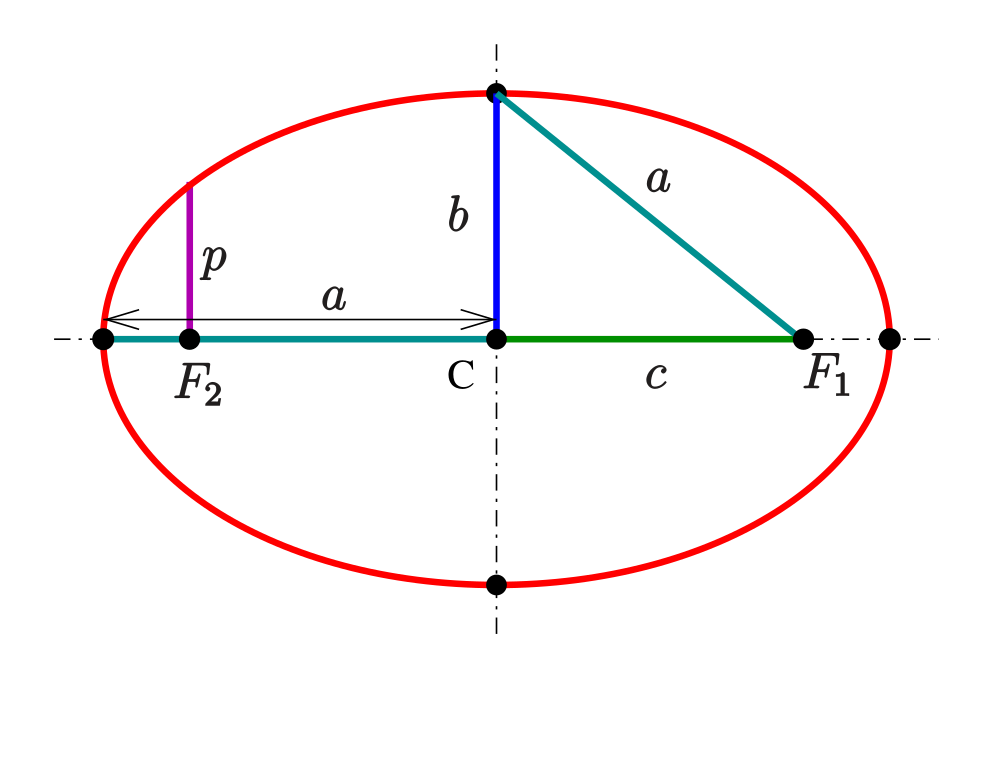
\includegraphics[width=.9\linewidth]{images/Ellipse-param.svg.png}
\caption{Image Courtesy: \href{https://commons.wikimedia.org/wiki/File:Ellipse-param.svg}{Wikipedia}}
\end{figure}
\end{column}

\begin{column}{.6\columnwidth}
Standard form
\begin{align}
  \notag
  f\left( \begin{matrix}x\\y\end{matrix} \right)
  &= \frac{x^2}{a^2} + \frac{y^2}{b^2} - 1 = 0
\end{align}

Parametric Form
\begin{align}
  \notag
  f(t;a,b) &= \begin{bmatrix}
    a\cos t \\ b \sin t
  \end{bmatrix}
\end{align}
\end{column}
\end{columns}
\end{frame}


\section{mid-point algorithm}
\label{sec:org33cbcf2}

\subsection{Fundamentals}
\label{sec:orgf9eee31}

\begin{frame}[label={sec:org26988b7}]{problem}
In a quantised (pixelated or discrete) 2d plane, find
the set of points that visually approximate a given
curve, say a straight line or a conic.
\end{frame}

\begin{frame}[label={sec:org40379aa}]{method}
\begin{columns}
\begin{column}{.5\columnwidth}
Iteratively, increment along one axes, \\[0pt]
with respect to which, the slope of the curve is
gentle.

{\vspace{\baselineskip}}
Decide whether it is required to increment along the
perpendicular axis or not.

{\vspace{\baselineskip}}
Increment if required.
\end{column}
\end{columns}
\end{frame}

\begin{frame}[label={sec:org21d6b70}]{example}
\begin{center}
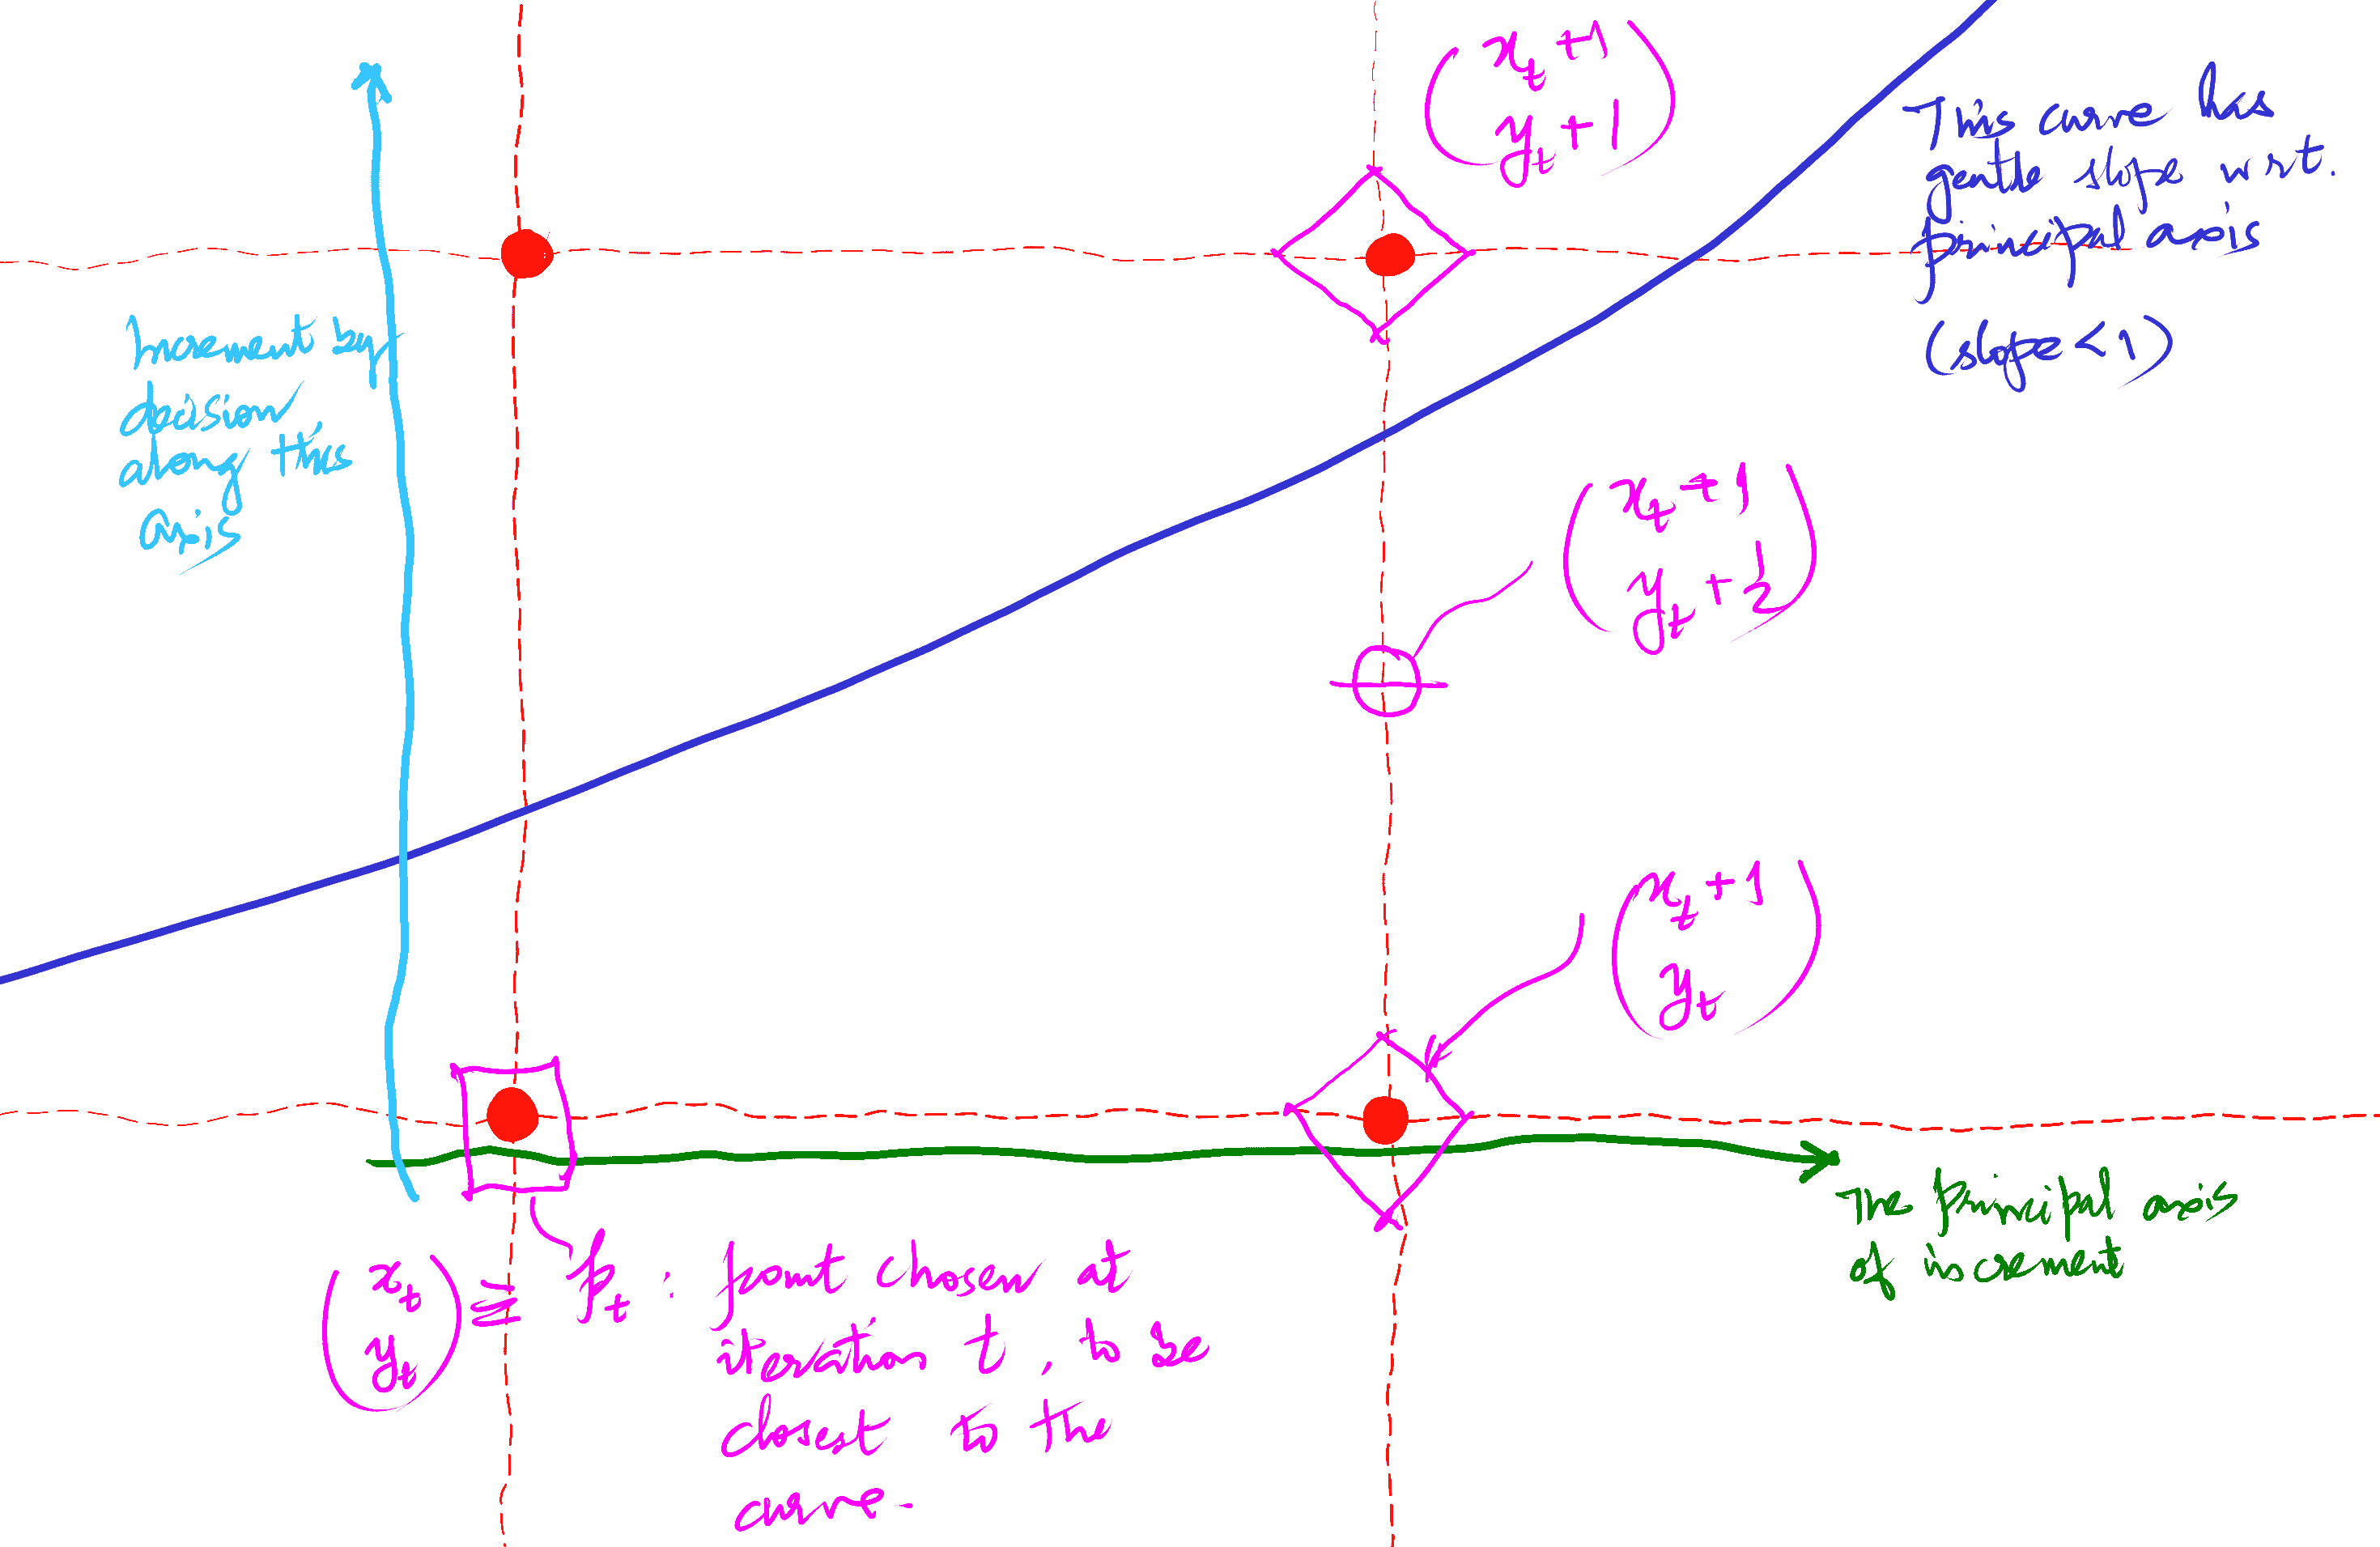
\includegraphics[width=0.65\linewidth]{images/basic-midpoint-algo.png}
\end{center}
\end{frame}
\end{document}
